\chapter{Oszthatlan közösen készített programok}\label{chap:oszthatlan_kozos_dolgok}


\section{A nyelvi séma}

\noindent

A JavaScriptSchéma egy UML Diagramhoz hasonlító schéma. Jelen esetben a Visual Paradigm alkalmazással szerkeszthető.
A felépítése a következőképpen alakul:

\begin{figure}[!htbp]
      \caption{JavaScriptSchema struktúrális felépítése}\label{fig:JavaScriptSchema_struktura}
      \centering
      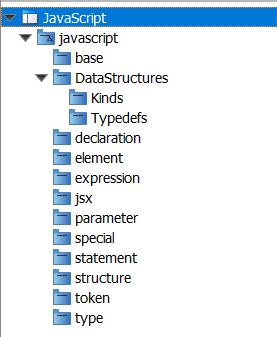
\includegraphics[width=0.4\textwidth]{JavaScriptSchema_struktura.png}
\end{figure}

\Aref{fig:JavaScriptSchema_struktura} ábrán a következő struktúra figyelhető meg: ProjektNév/Model/Packagek.
A projekt neve a JavaScript, ezen belül található egy model, amit javascript-nek hívnak. A modellen belül találhatóak meg a packagek.
A Packagek nem véletlenül így lettek elnevezve. Az alábbi hivatkozáson található meg, hogy milyen logika alapján neveztük el a packageket:~\cite{typescript-eslint}
Nem feltétlenül muszáj több packaget létrehozni, ez csupán az átláthatóság és a könnyen bővíthetőség céljából lett így megvalósítva.
Követtük a typescript-eslint githubon lévő projekt struktúrális logikáját, de több helyen is eltértünk tőle, mivel a mi projektünk másabb, illetve speciális megoldásokat igényelt egyes helyeken.
A következő oldalakon bemutatom a packagek felépítését néhány egyszerűbb példán szemléltetve.
A packagek a következőképpen épülnek fel:
\begin{figure}[!htbp]
      \caption{A base package felépítése}\label{fig:base_vpp}
      \centering
      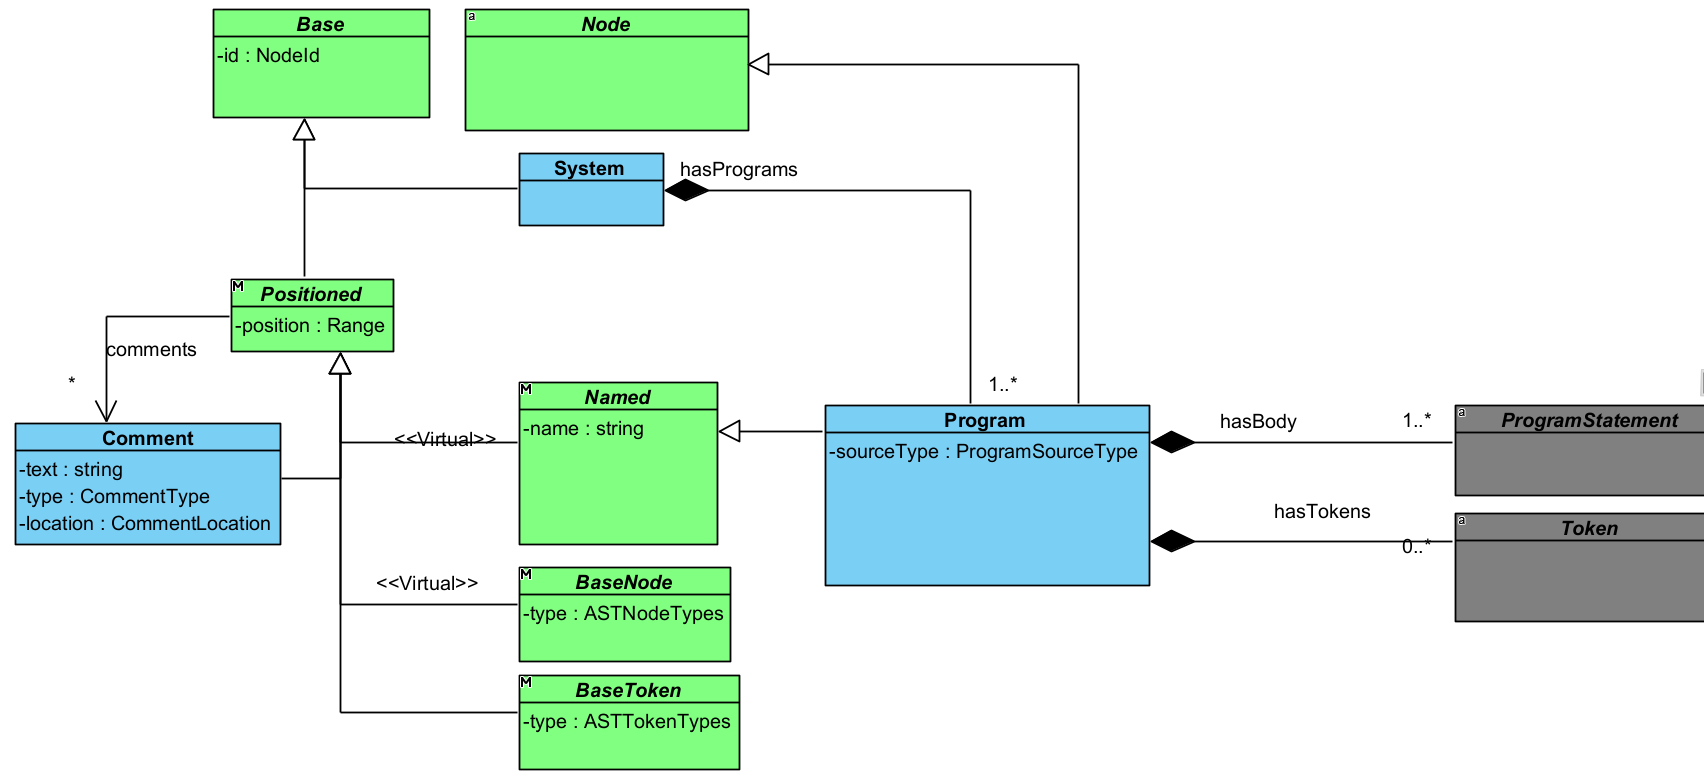
\includegraphics[width=0.9\textwidth]{base_vpp.png}
\end{figure}

\Aref{fig:base_vpp} ábrán különböző osztályok láthatóak. A Base osztály mindennek az alapja, ebből öröklődik minden más.
Látható, hogy egy id attribútummal rendelkezik, aminek a típusa NodeId.
A zöld háttérszínű osztályok az absztrakciót jelentik. Az asg fileban jelentősége, illetve a schéma szerkeszthetősége és olvashatósága miatt van így jelezve.
A szürke háttérszínű osztályok pedig csupán annyit jelentenek, hogy más packageben lettek definiálva.
A kék a default, normális osztályt jelölik.
A Positioned és a System származik le a Baseből, értelemszerűen a system az maga a program lesz.
A Positioned az azért absztrakt, mivel majd ebből fognak leszármazni a kisebb osztályok, mint például az expression, statement és a többi.
A Positioned osztálynak van egy attribútuma, a poisition, ami egy Range típus. Emellett még tartozhatnak hozzá kommentek is.
A komment egyaránt leszármazik a positioned-ből, ezzel garantálva azt, hogy a kommentnek van pozíciója.
Látható, hogy a kommentnek van egy text, type és location attribútuma. A CommentType és a CommentLocation a DataStructures-ben van definiálva.
Emellett a Named, BaseNode és a BaseToken származik le a Positionedből. A Named osztály azt jelenti, hogy egy nodenak van-e name attribútuma vagy sem.
A BaseNodeból és a BaseTokenből fog nagyon sok minden leszármazni aminek van typeja.
Végül, megtalálható a Program osztály, aminek van name attribútuma, mivel Named-ből származik le, és van Systeme. Az 1..* jelenti azt, hogy legalább 1 Systeme van, de lehet több is.
A hasPrograms-nak majd máshol lesz jelentősége, a mi esetünkben majd a javascriptben.
Tetszőlegesen el lehet nevezni, de konzisztencia miatt, minden attribútum ami osztály (és nem a DataStructuresben azon belül is a Kindsban van definiálva, hanem van neki egy osztály, mint pl Comment)
azt a hasOsztály névvel fogjuk ellátni.
A ProgramSourceType is a Kinds packageben van definiálva, ami csupán azt mondja meg, hogy az adott program vagy script vagy module típusú.
A base package nem követi a typescript-eslint githubon lévő projekt base mappáját, ez teljesen egyedi, átememeltük az egészet apróbb módosítással az előző projekt verzióból.

\noindent

A base packagen kívül bemutatom a declaration packaget, hogy lássuk milyen logikát követtünk a megírás során.
Ezen belül is az ExportAllDeclaration bemutatása:

\Aref{lst:ExportAllDeclaration} kódrészlet így lett megvalósítva a JavaScriptSchémában:
\begin{lstlisting}[caption={ExportAllDeclaration typescriptes megvalósítása},label={lst:ExportAllDeclaration}, language={JavaScript}]
export interface ExportAllDeclaration extends BaseNode {
      type: AST_NODE_TYPES.ExportAllDeclaration;
      assertions: ImportAttribute[];
      exported: Identifier | null;
      exportKind: ExportKind;
      source: StringLiteral;
}
\end{lstlisting}

\begin{figure}[!htbp]
      \caption{A declaration package felépítése}\label{fig:declaration_vpp}
      \centering
      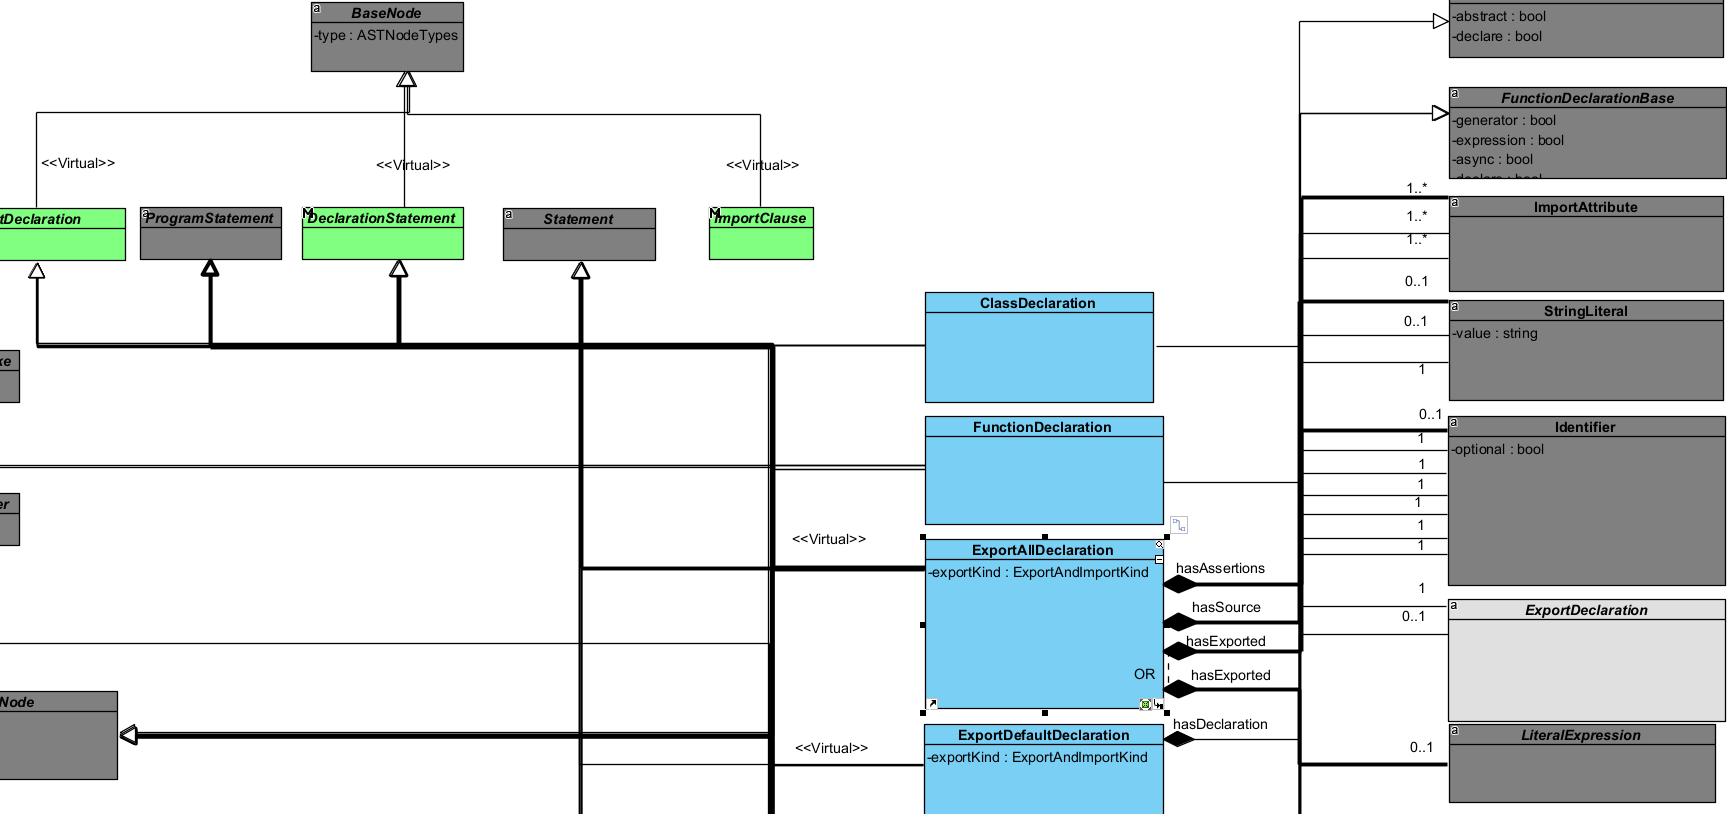
\includegraphics[width=0.8\textwidth]{declaration.png}
\end{figure}

\Aref{fig:declaration_vpp} ábrán látható az, hogy minden a BaseNodeból származik. \Aref{lst:ExportAllDeclaration} kódrészletben ez az extends BaseNode.
Itt maga a declaration osztály az a DeclarationStatement névre hallgat, csupán azért, mert követtük a typescriptes kódot. A főbb osztályok a BaseNode alatt találhatóak.
Jobb oldalt a sötétszürke és a világosszürke osztályok azok az attribútumok.
Ebben az esetben az ExportAllDeclaration osztály leimplementálását mutatom be a JavaScriptSchemában.
Az ExportAllDeclaration öröklődik a Statement, DeclarationStatement, Node és a ProgramStatementből.
Ezeket az öröklődéseket ugyanúgy a typescript-eslint githubról néztük, unions mappában találhatóak el.
Ezáltal megkapja az összes szülőnek a tulajdonságait. A DeclarationStatement öröklődik a BaseNodeból, ami azt jelenti, hogy a BaseNode tulajdonságait is megkapja az ExportAllDeclaration.
A BaseNode ugye meg származik a Positionedből, ez látható \aref{fig:base_vpp} ábrán.
Emiatt az ExportAllDeclaration-nek lesz pozíciója, kommentje és NodeId-ja is.
Assertions attribútum típusa az ImportAttribute, látható, hogy egy tömböt vár, ezért 1..* a multiplicityje.
Exported attribútumnál egy Identifier típusú attribútumot vár, itt mi kiegészítettük még egy LiteralExpressiönnel is, ami maga a Literal.
A vagyolást egy OR-al jeleztük a JavaScriptSchemában.
Mivel lehet null-is, ezért 0..1 a multiplicity, szóval vagy 0 vagy 1.
Az ExportKind az a Kindsban található meg, így szimplán csak arra hivatkozunk, mint ExportAndImportKind.
Végül a source attribútuma egy StringLiteral, nálunk is így szerepel.
Természetesen ami sötétszürkével van jelölve, az máshol létre van hozva és vannak neki attribútumai.
A világosszürke annyit jelöl, hogy ebben a packageben lett létrehozva az osztály, de láthatóság szempontból többször szerepel, mivel lehet attribútum is.
Így lett minden egyes osztály felépítve, természetesen \Aref{fig:declaration_vpp} ábra csak egy részlete a declaration packagenek, ennél jóval nagyobb.
Vannak úgynevezett gyűjtő osztályok is, mint pl a Statement, ezekre azért van szükség, mert majd később ha le lett generálva minden, akkor tudjunk majd vizsgálni különböző nodeokra, mint például az isStatement.

\noindent

Sokat említettem a DataStructurest. Hadd mutassam be egy példán keresztül, hogy ez hogy néz ki.

\begin{figure}[!htbp]
      \caption{A DataStructures packageben a Kind package felépítése}\label{fig:data_structures_kinds}
      \centering
      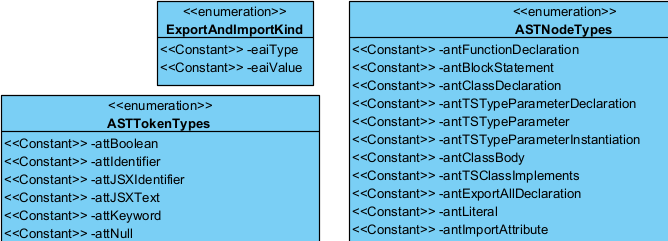
\includegraphics[width=0.8\textwidth]{data_structures.png}
\end{figure}

A DataStructures packageben található 2 package, ez \aref{fig:JavaScriptSchema_struktura} ábrán látható. Ebből a Kinds packaget mutatom be.
\Aref{fig:data_structures_kinds} ábrán látható egy kis szelet a Kinds packageből.
Enumok találhatóak ebben a packageben.
Például ha az ExportAndImportKind-ot adjuk meg típusnak az egyik attribútumnak, akkor az lehet vagy eaiType vagy eaiValue.
Minden constant előtt van 3 karakter, ez azért szükséges, mert később ezekkel még foglalkozni fogunk.

\noindent

A JavaScriptSchema magában még semmit sem csinál. Először ki kell exportálni az egész projectet xml formátumba.
Ezután az xml filet átkonvertáljuk egy asg filera. Ez úgy történik, hogy a JavaScript Analyzer projektnek van egy kisebb alprojektje, amit UmlToAsg-nek hívnak.
Ez a java kód átkonvertálja az xml fileban lévő adatot egy asg fileba. Jobban nem térnék ki az UmlToAsg projektre, mivel nem szerkesztettük.
Az UmlToAsg projektet a SchemaGenerator generálta le. A SchemaGenerator c++ nyelven megírt program. Több mindent is generál c, c++, vagy java nyelven.
Ez a projekt is az Analyzer JavaScript  alprojektei közé tartozik.
A file elején a következő található meg:
\begin{lstlisting}[caption={Asg file első sorai},label={lst:asg_file_eleje}, language={JavaScript}]
NAME = javascript;
APIVERSION = 0.3.1;
BINARYVERSION = 0.3.1;
CSIHEADERTEXT = JavaScriptLanguage;
\end{lstlisting}

A verziókat kézzel tudjuk átírni abban a fileban ami generálja ezt, ez egy c++ file, a SchemaGeneratorban található meg.
Ezután a Kinds mappa tartalmát írja bele a következőképpen:
\begin{lstlisting}[caption={Asg file kind},label={lst:asg_file_kinds}, language={JavaScript}]
KIND ASTNodeTypes (ant) {
      FunctionDeclaration;
      BlockStatement;
      ClassDeclaration;}
\end{lstlisting}
Az a 3 karakter amit minden constant elé tettünk azt kitette paraméterbe és csak az utáni stringet írta át. Ugyanígy van a többi kindnál is.
Ha az összes kindot beleírta, akkor kezdi írni sorban a többi packaget. \Aref{fig:JavaScriptSchema_struktura} alapján megy sorba.
Példának a declaration packaget mutatom be, azon belül is az ExportAllDeclaration-t.
\begin{lstlisting}[caption={Asg file ExportAllDeclaration},label={lst:asg_file_export_all_declaration}, language={JavaScript}]
SCOPE declaration {

      NODE DeclarationStatement : virtual base::BaseNode [ABSTRACT] {
      }

      NODE ExportAllDeclaration : DeclarationStatement, statement::Statement, virtual statement::ProgramStatement, special::Node {
            ATTR ExportAndImportKind exportKind;
            EDGE TREE 1 hasExported (expression::Identifier | expression::LiteralExpression);
            EDGE TREE 1 hasSource (structure::StringLiteral);
            EDGE TREE * hasAssertions (special::ImportAttribute);
      }
}
\end{lstlisting}
Látható, hogy a Packaget SCOPE-nak értelmezi, és ezen belül NODE-ok találhatóak.
A Nodeoknak ATTR és EDGE TREE van. A vagyolás is látható.
Az öröklődik egy kettőspont után, felsorolás szerűen írta át, ha valami másból származik, akkor packageNev::osztalyNev szerint.
Az kapott ATTR jelölést ami a Kinds-ban megtalálható vagy egy szimpla típus (mint pl string, int).
Minden mást EDGE TREE-nek nevezett el. Az Edge tree utáni szám vagy csillag az a multiplicitást jelenti.
Ha 1es, akkor a multiplicitás 0..1, ha *, akkor vagy 0..* vagy 1..* a multiplicitás.
\Aref{fig:declaration_vpp}as ábrán látható, hogy mit hogyan írt át.

\section{A nyelvi séma átírása}

\noindent

A JSAN a JavaScriptSchemára épül. Ha valamit meg akarunk változtatni gyökerestül a JSANba, akkor a schémát is változtatni kell.
Azt elérni, hogy javascript mellett még typescriptes kódokat is elemezzen a JSAN, ahhoz gyökerestül meg kellett változtatni a JavaScript Analyzert.
Az előző JavaScriptSchema (ami csak javascriptet elemzett) az a javascript hivatalos oldala alapján készült. Ami ábrák fentebb megtalálhatóak, azok már az átírt schémából vannak.
Több opció is volt, hogy most vagy legyen átírva a schéma, vagy legyen egy külön typescriptre is írva.
Végül rájöttünk, hogy ha van egy typescriptes schémánk, az képes javascriptet ugyanúgy elemezni ha megfelelően van lefejlesztve.
Így egy schémát fejlesztettünk le. Az előző schéma átláthatatlan volt, ezért úgy döntöttünk, hogy majdnem a nulláról újraírjuk.
Egyedül a base packaget emeltük át a régiből, BaseNode-al és BaseTokennel kibővítve (\Aref{fig:base_vpp} ábrán látható).
Emellett el kellett dönteni, hogy milyen struktúrát kövessünk, ami jól átlatható és később könnyebben bővíthető.
Végül a typescript-eslint official github alapján haladtunk. Annyi változtatással, hogy ami nekik a base mappában volt, mi arra létrehoztunk egy külön structure packaget.
Mindenhez készítettünk dokumentációt, jól érthetően leírtuk, hogy mit miért kellett csinálni.
Mivel minden is egymásra épül a typescriptes schémában, ezért nem tudtuk tesztelni minden egyes package után, hogy működik-e vagy sem.
Mint például, látható \aref{lst:asg_file_export_all_declaration} kódrészleten, hogy az ExportAllDeclaration mennyi mindenből származik le vagy mennyire sok attribútuma van.
Az ExportAllDeclaration egyik attribútuma, az assertions típusa az ImportAttribute. Ahhoz, hogy jól észrevegye az ExportAllDeclarationt az Analyzer, ahhoz jól le kellett fejleszteni az ImportAttributet.

\begin{lstlisting}[caption={ImportAttribute},label={lst:asg_file_import_attribute}, language={JavaScript}]
export interface ImportAttribute extends BaseNode {
      type: AST_NODE_TYPES.ImportAttribute;
      key: Identifier | Literal;
      value: Literal;
}
\end{lstlisting}
Ahhoz, hogy az ImportAttributet letudjuk fejleszteni a schémában, ahhoz le kell fejleszteni az Identifiert, és a Literalt.
Kicsit összetett, hogy mi minden épül egymásra. Ebből adódik a következő alfejezet mondandója is.

\section{Nehézségek, problémák}

\noindent

A schéma átírása során több nehézségbe is ütköztünk.
A legelső nehézség az a Visual Paradigm program korrekt használata volt.
Egy kisebb időbe tellett rájönni arra, hogy egy adott classnak hogyan kell megváltoztatni a háttérszínét, packagek közötti mozgást, hogyan kell egy adott classra hivatkozni ami másik packageben volt.
Ezután ami szerintem a legnagyobb nehézség volt, az az, hogy nem volt dokumentáció az előző schémához.
Mindent nekünk kellett kitalálni, hogy mit miért csináltak az előző fejlesztők. Akik ezt a schémát fejlesztették le, ők már nem foglalkoztak ezzel, és más nem nagyon mélyedt bele ebbe az egészbe azóta.
A következő nagyobb nehézség, az az volt, hogy összehozzunk egy olyan schémát ami működőképes, és az analyzer ezt tudja is használni.
Előző alfejezetben említettem, hogy egy adott classt (mint például ExportAllDeclaration) lefejlesszünk, ahhoz sok minden mást is le kell fejleszteni, amihez meg még több minden kellett.
Ebből adódóan tesztelni nagyon nem tudtunk, mivel az egésznek működnie kellett ahhoz, hogy az analyzer egyáltalán lefusson.
Mivel mi majdnem nulláról írtuk újra, ez volt a hátrány.
Amikor elérkeztünk ahhoz az állapothoz, hogy mindenre rámondjuk azt, hogy működik, akkor jött egy nagyobb probléma.
Valahol Segmentation Fault-ot kapott a program, és nem nagyon tudtuk ezt debugolni.
Több sejtésünk is volt, hogy mi lehet a baj. Emiatt az egész schémát át kellett nézni alaposan, hogy hol vétettünk hibákat.
Sok helyen voltak pontatlanságok, rossz osztályból származtattunk le, rossz típus volt megadva attribútumnak. Ezeket mind kijavítottuk, de most már más hibát kaptunk.
A JavaScript Analyzerben kiderítettük, hogy pontosan hol szállt el a program.
A Literal volt a hiba, mivel ezt nem a github alapján írtuk meg, hanem egyedi ötlettel. Előző schémában is máshogy volt megoldva.
\begin{figure}[!htbp]
      \caption{A DataStructures packageben a Kind package felépítése}\label{fig:literal}
      \centering
      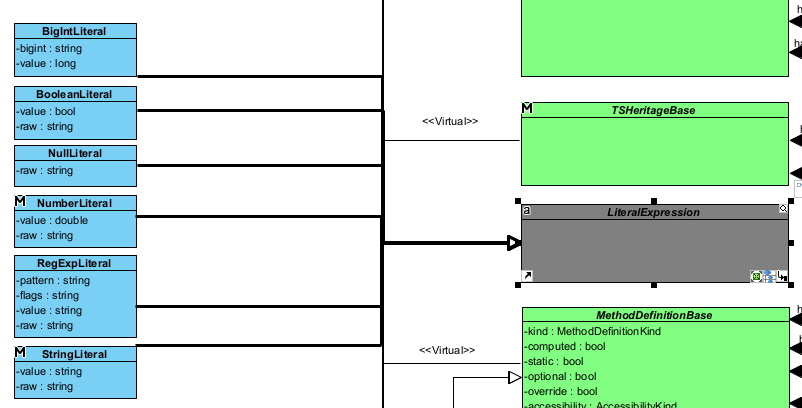
\includegraphics[width=0.8\textwidth]{literal.png}
\end{figure}

\Aref{fig:literal} ábrán látható, hogy a LiteralExpressionből (Ami a Literal) több literal is öröklődik.
\begin{lstlisting}[caption={Literal},label={lst:asg_file_literal}, language={JavaScript}]
export interface LiteralBase extends BaseNode {
  type: AST_NODE_TYPES.Literal;
  raw: string;
  value: RegExp | bigint | boolean | number | string | null;
}
\end{lstlisting}
Próbáltuk úgy megoldani, hogy 4 vagyolással 4 különböző literál tartalmazza, de az analyzerben máshogy kezeltük le a literalt, mint nodeot.
Ezért a tartalmazás helyett inkább örököltettünk a literalból, így megoldva ezt a problémát.
Még az is probléma volt, hogy volt egy LiteralBaseünk, amiből származott ez az 5 literal. A LiteralBase származott a LiteralExpressionből, de valamiért Segmentation fault lett a vége ha így próbáltuk megoldani.
Ezért a LiteralBase-t kivettük, és LiteralExpressionből származik minden literal.
Végül még az volt a nehézség, hogy kódrészletet keressünk az analyzernek, amin le tudjuk tesztelni, hogy az analyzer jó outputot ad-e.

\noindent

Mivel nem nagyon volt typescriptes háttértudásunk, először a typescriptet kellett átnézni, hogy mit hogyan tudunk megvalósítani.
Emellett még a javascriptes outputokat is át kellett nézni, mivel a mi célunk a fejlesztés volt. A jelenlegi javascriptes projektekre ugyanolyan eredményt adott, sőt néhány helyen jobbat is, mert az előző schémában is voltak pontatlanságok.
A typescriptes projektek nagy részét tudja elemezni az analyzer, de közel sem tökéletes, mivel egyfolytában kellene fejleszteni a schémát, mivel a typescript nem annyira régi.


